% This must be in the first 5 lines to tell arXiv to use pdfLaTeX, which is strongly recommended.
\pdfoutput=1
% In particular, the hyperref package requires pdfLaTeX in order to break URLs across lines.

\documentclass[11pt]{article}\usepackage[]{graphicx}\usepackage[]{color}
% maxwidth is the original width if it is less than linewidth
% otherwise use linewidth (to make sure the graphics do not exceed the margin)
\makeatletter
\def\maxwidth{ %
  \ifdim\Gin@nat@width>\linewidth
    \linewidth
  \else
    \Gin@nat@width
  \fi
}
\makeatother

\definecolor{fgcolor}{rgb}{0.345, 0.345, 0.345}
\newcommand{\hlnum}[1]{\textcolor[rgb]{0.686,0.059,0.569}{#1}}%
\newcommand{\hlstr}[1]{\textcolor[rgb]{0.192,0.494,0.8}{#1}}%
\newcommand{\hlcom}[1]{\textcolor[rgb]{0.678,0.584,0.686}{\textit{#1}}}%
\newcommand{\hlopt}[1]{\textcolor[rgb]{0,0,0}{#1}}%
\newcommand{\hlstd}[1]{\textcolor[rgb]{0.345,0.345,0.345}{#1}}%
\newcommand{\hlkwa}[1]{\textcolor[rgb]{0.161,0.373,0.58}{\textbf{#1}}}%
\newcommand{\hlkwb}[1]{\textcolor[rgb]{0.69,0.353,0.396}{#1}}%
\newcommand{\hlkwc}[1]{\textcolor[rgb]{0.333,0.667,0.333}{#1}}%
\newcommand{\hlkwd}[1]{\textcolor[rgb]{0.737,0.353,0.396}{\textbf{#1}}}%
\let\hlipl\hlkwb

\usepackage{framed}
\makeatletter
\newenvironment{kframe}{%
 \def\at@end@of@kframe{}%
 \ifinner\ifhmode%
  \def\at@end@of@kframe{\end{minipage}}%
  \begin{minipage}{\columnwidth}%
 \fi\fi%
 \def\FrameCommand##1{\hskip\@totalleftmargin \hskip-\fboxsep
 \colorbox{shadecolor}{##1}\hskip-\fboxsep
     % There is no \\@totalrightmargin, so:
     \hskip-\linewidth \hskip-\@totalleftmargin \hskip\columnwidth}%
 \MakeFramed {\advance\hsize-\width
   \@totalleftmargin\z@ \linewidth\hsize
   \@setminipage}}%
 {\par\unskip\endMakeFramed%
 \at@end@of@kframe}
\makeatother

\definecolor{shadecolor}{rgb}{.97, .97, .97}
\definecolor{messagecolor}{rgb}{0, 0, 0}
\definecolor{warningcolor}{rgb}{1, 0, 1}
\definecolor{errorcolor}{rgb}{1, 0, 0}
\newenvironment{knitrout}{}{} % an empty environment to be redefined in TeX

\usepackage{alltt}

% Remove the "review" option to generate the final version.
\usepackage{acl} % [review]{acl}

% Standard package includes
\usepackage{times}
\usepackage{latexsym}
\usepackage[normalem]{ulem}

% For proper rendering and hyphenation of words containing Latin characters (including in bib files)
\usepackage[T1]{fontenc}
% For Vietnamese characters
% \usepackage[T5]{fontenc}
% See https://www.latex-project.org/help/documentation/encguide.pdf for other character sets

% This assumes your files are encoded as UTF8
\usepackage[utf8]{inputenc}

% This is not strictly necessary, and may be commented out,
% but it will improve the layout of the manuscript,
% and will typically save some space.
\usepackage{microtype}

\usepackage{gb4e}\noautomath
\usepackage{amsmath}\noautomath

\usepackage[edges]{forest}

\def\citeapos#1{\citeauthor{#1}'s (\citeyear{#1})} 

% If the title and author information does not fit in the area allocated, uncomment the following
%
%\setlength\titlebox{<dim>}
%
% and set <dim> to something 5cm or larger.

\title{A multinomial processing tree model of RC attachment}

% Author information can be set in various styles:
% For several authors from the same institution:
% \author{Author 1 \and ... \and Author n \\
%         Address line \\ ... \\ Address line}
% if the names do not fit well on one line use
%         Author 1 \\ {\bf Author 2} \\ ... \\ {\bf Author n} \\
% For authors from different institutions:
% \author{Author 1 \\ Address line \\  ... \\ Address line
%         \And  ... \And
%         Author n \\ Address line \\ ... \\ Address line}
% To start a seperate ``row'' of authors use \AND, as in
% \author{Author 1 \\ Address line \\  ... \\ Address line
%         \AND
%         Author 2 \\ Address line \\ ... \\ Address line \And
%         Author 3 \\ Address line \\ ... \\ Address line}

\author{Pavel Logačev \\
  Boğaziçi University \\
  Department of Linguistics \\
  34342 Istanbul, Turkey \\
  \texttt{pavel.logacev@gmail.com} \\\And
  Noyan Dokudan \\
  Boğaziçi University \\
  Department of Linguistics \\
  34342 Istanbul, Turkey \\
  \texttt{noyan.dokudan@gmail.com} \\}


\IfFileExists{upquote.sty}{\usepackage{upquote}}{}
\begin{document}
\maketitle
\begin{abstract}
Studies in the field of sentence processing often use a variant of a discrete choice task to determine speakers' understanding of ambiguous sentences. We discuss a largely neglected source of potential bias and variability that may affect the results of such experiments. We propose an analysis method based on multinomial processing tree models \citep{BatchelderRiefer:1999} which corrects for this bias and allows for a separation of parameters of theoretical importance from nuisance parameters. We test two variants of the MPT-based model. We further demonstrate that this method can provide deeper insight into the processes underlying participants' answering behavior as well as their attachment preferences.
\end{abstract}

\section{Introduction}

One of the key questions in the field of sentence processing has been: \textit{What does the human sentence processing mechanism do when confronted with an ambiguity?} A variety of different proposals for a variety of disambiguation strategies have been made over the years, such as the Garden-path Theory \citep{Frazier:1987}, the Tuning Hypothesis \citep{CuetosEtAl:1996}, the Competition-Integration Model \cite{McRaeEtAl:1998} and many others. 
Their diverging predictions have led to a large body of empirical research documenting, among other things, substantial cross-linguistic variation in the interpretation of ambiguous sentences: 
For instance, \citet{CuetosMitchell:1988} compared the RC attachment preferences of English and Spanish speakers in ambiguous sentences like (\ref{Ex1}) and (\ref{Ex2}), in which the relative clause \textit{'who had the accident'} can attach either to the NP headed by the first noun (N1, \textit{'daughter'}) or to the NP headed by the second noun (N2, \textit{'colonel'}).\footnote{In order to avoid any ambiguity in the context of typologically diverse languages, we will refer to the two interpretation options as \textit{N1 attachment} and \textit{N2 attachment}, with N1 and N2 referring to the order of occurrence of the noun phrases head nouns instead of the more common terms \textit{high attachment} and \textit{low attachment}.} 

Cuetos and Mitchell presented Spanish-speaking and English-speaking participants with ambiguous sentences like (\ref{Ex1}) and (\ref{Ex2}) and asked them to answer comprehension questions like \textit{`Who had an accident?'}. Participants' responses indicated that English sentences like (\ref{Ex1}) received an N2 interpretation in $61\%$ of the cases, while their Spanish counterparts like (\ref{Ex2}) received an N1 interpretation in $72\%$ of the cases. The authors interpret this finding as an argument for a universal parsing strategy in the resolution of RC attachment ambiguities.

\begin{exe}
\ex \label{Ex1} The journalist interviewed the daughter$_{N1}$ of the colonel$_{N2}$ [who had an accident].
\end{exe}

\begin{exe}
\ex \label{Ex2} 
\gll El periodista entrevisto a la hija$_{N1}$ del coronel$_{N2}$ [que tuvo el accidente]. \\
     The journalist interviewed to the daughter {of the} colonel [who had an accident]. \\
\end{exe}

Although the speakers' disambiguation strategy seems to be at least in part determined by language-specific factors, a variety of other factors appear to influence ambiguity resolution in RC attachment.
In an off-line questionnaire study, \citet[inter alia]{GilboyEtAl:1995} demonstrated a substantial influence of construction type. They asked participants to indicate which of the two available noun phrases was modified by the RC in several constructions. They found that the percentage of N2 attachment responses ranged between approximately $20\%$ to $70\%$ for their English sentences, and between $10\%$ to $80\%$ for their Spanish sentences. \citet{GrilloEtAl:2015} also conducted a two-alternative forced choice (2AFC) task in which English speakers choose between N1 and N2 as the attachment sites for the RC to indicate their interpretation of sentence. They showed that English speakers, who had previously been claimed to prefer N2 attachment, preferred N1 attachment in more than $50\%$ of the cases when a small clause reading was possible.

% NOTE: This might be too much away from methods, towards the actual question of attachment 
%\citet{MaiaEtAl:2007} discussed the effect of the task used to examine RC attachment preferences on the variation regarding RC attachment preference observed in the same language. Speakers of Brazilian Portuguese who took part in their self-paced reading experiment spent more time in reading the RC verb when the structure forced them to choose high attachment than when it forced them to choose the low attachment reading, suggesting an *initial* low attachment preference. Nevertheless, the error rates of the answers to comprehension questions were higher for low attachment structures (approximately $30\%$) than high attachment structures (approximately $15\%$), which Maia et al. take as an indicator of an offline preference towards high attachment. They also review other studies to support their claim that when a speeded task is employed higher rates of low attachment are observed in the Roman languages that favor high attachment in offline tasks.

RC attachment preferences have also been studied in Turkish, where the order of RC and complex noun phrase is reversed. In a questionnaire study with sentences like (\ref{Ex3}), \citet{Kirkici:2004} found that animacy may affect attachment preferences such that when both NPs are [+human], there are no significant difference between the proportions of the N1 and N2 attachment, while an N1 attachment manifested when both NPs were [-human]. Contrary to this finding, \citet{Dinctopal-Deniz:2010} found an across-the-board preference for N1 attachment in Turkish. In her questionnaire study, monolingual Turkish speakers read Turkish sentences with ambiguous RC attachment and answered questions about those by indicating one of two options on each trial. The results of this study showed that participants preferred N1 attachment over N2 attachment ($66\%$ and $34\%$, respectively). %More recently, \citet{Akal:2021} conducted two experiments with Turkish sentences with ambiguous RC attachment. The results of their experiments indicate an overall N1 attachment preference ($79.5\%$ percent in Experiment 1 and $60.8\%$ percent in Experiment 2).

\begin{exe}
\ex \label{Ex3} \gll Şoför [şehir merkezinde     oturan]$_{RC}$ profesörün$_{N1}$ sekreterini$_{N2}$ gördü. \\
                     driver {in the city center} living  professor's secretary saw \\
                    \textit{'The driver saw the secretary of the professor who was living in the city center.'}
\end{exe}



\section{The Role of Guessing}

What most of the above studies of RC attachment preferences have in common is that they use some variant of a discrete choice task, in which participants select one of two response options to indicate their interpretation of the ambiguity. The relative proportion of responses indicating N1 and N2 attachment, respectively are interpreted as estimates of the magnitude of N1 or N2 attachment.
A potential complication in interpreting the percentages of N1 and N2 responses in this way is that participants' responses may not always reflect their interpretation. It appears quite likely that, on some trials, participants process the sentence only partially or fail to pay attention to it altogether. In such cases, participants' question responses must be based on an incomplete or nonexistent representations, 
and are more likely to resemble guesses than informed responses.

Evidence for such incomplete processing comes from the widely known fact that participants' accuracy in experimental tasks is often far from perfect, even for relatively simple tasks such as acceptability judgments: For example, \citet{DillonWagers:2019} found in an \textit{off-line} acceptability judgment study that ungrammatical sentences like (\ref{E4}) are judged acceptable on $18\%$ of the trials. 
Since it appears unlikely that sentences like \ref{E4} are considered grammatical and interpretable when fully processed, the explanation for such responses must lie in their incomplete processing followed by guessing.

\begin{exe}
\ex \label{E4} *Who do you think that the new professor is going to persuade anyone?
\end{exe}

One way of conceptualizing a simple generative model of erroneous responses in relatively simple tasks is to assume that at least some participants on some occasions fail to pay attention to the stimulus, and as a result, select a random response. 

If so, the relation between the probability of response \textit{X}  being actually preferred to alternative responses ($p_X$) and the probability of observing response \textit{X} ($p_X'$) can be formalized as in equation \ref{eq:EqEx1}: 
$p_{X}'$ is the weighted average of (i) the probability of \textit{X} being preferred to the alternative when the stimulus is fully processed ($p_{X}$) and (ii) the probability of selecting \textit{X} when the stimulus is not attended ($g_X$), where $a$ is the probability of attending to the stimulus.

\begin{equation}
p_{X}' = a \cdot p_{X} + (1-a) \cdot g_X
\label{eq:EqEx1}
\end{equation}

Given that participants in most if not all psycholinguistic tasks produce a sizeable amount of erroneous responses, it appears \textit{a priori} quite plausible that such mechanisms are also at play in attachment preference studies. This means that empirical estimates of attachment preferences ($p_X'$) are likely to be (i) \textit{biased} towards the guessing parameter $g_X$ to a degree determined by $a$, and (ii) are likely to \textit{vary between studies} as a function of both, $a$ and $g_X$.

% to-do: Make sure to connect it to the typical 2AFC paradigm later.
In the following, we propose a method for disentangling the contributions of attachment preferences and guessing using multinomial processing tree models \citep[MPT;][]{ErdfelderEtAl:2009, BatchelderRiefer:1999} based on response patterns in unambiguous baseline sentences. We present two alternative MPT models for the task of answering polar comprehension questions about sentences with ambiguous and unambiguous RC attachment in two languages, English and Turkish.


\section{Experiments}

To evaluate our method, we used question-answering data from two experiments in which participants read sentences with ambiguous and unambiguous RC attachments and answered polar comprehension questions about them.

\subsection{Experiment 1}
We used the question-answering data from the RC questions condition in \citeapos{SwetsEtAl:2008} self-paced reading experiment in English (N=48), in which participants read sentences like (\ref{SwetsExSentence}) in three attachment conditions and answered comprehension questions about RC attachment which were similar to (\ref{SwetsExQuestion}) on every trial. All comprehension questions required a \textit{'yes'}/\textit{'no'} answer. One-half of the questions asked whether the RC modified the noun phrase headed by N1, and the other half asked about N2.

RC attachment was disambiguated by means of gender (mis)match between the reflexive in the RC and the RC head noun. Each participant read 36 experimental sentences. Unambiguous sentences had correct answers, while the responses to ambiguous sentences indicate how readers disambiguated the sentence, thus reflecting their RC attachment preference.

Figure \ref{avg_perc} (left panel) shows the average percentages of \textit{'yes'} responses to comprehension questions by attachment condition and question type (question about N1 or N2).

\begin{exe}
\ex \label{SwetsExSentence} 
\begin{xlist}
    \ex \textsc{ambiguous attachment} \\
        The \uline{maid}$_{N1}$ of the \uline{princess}$_{N2}$ $[$who scratched \textit{herself} in public$]$ \ldots
    \ex \textsc{N1 attachment} \\
        The \uline{son}$_{N1}$ of the princess$_{N2}$ $[$who scratched \textit{himself} in public$]$ \ldots
    \ex  \textsc{N2 attachment}\\
        The son$_{N1}$ of the \uline{princess}$_{N2}$ $[$who scratched \textit{herself} in public$]$ \ldots
\end{xlist}
\ldots was terribly humiliated.
\end{exe}

\begin{exe}
\ex \label{SwetsExQuestion} \textsc{comprehension question} \\ 
    Did the maid/princess/son scratch in public?
\end{exe}


\subsection{Experiment 2}
The second set of question-answering data came from an unpublished self-paced reading experimental about RC attachment in Turkish (N=99). In an experiment design similar to Swets et al., participants read sentences like (\ref{TREx}). Because Turkish relative clauses are pre-nominal, the RC \textit{who hit each other} preceded the complex noun phrase \textit{the fans of the football players}. RC attachment of the  was disambiguated by the number marking of the head nouns as RCs with the reciprocal \textit{each other} can only modify plural noun phrases. The structure is ambiguous if both nouns are plural because they are both licit attachment sites for the RC. Participants were asked \textit{'yes'}/\textit{'no'} comprehension questions about RC attachment, like (\ref{TRQuestion}). The comprehension question asked about the event mentioned in the RC and whether one of the nouns was involved in that event.
Each participant read 42 experimental sentences. One-half of the questions asked whether the RC modified the noun phrase headed by N1, and the other half asked about N2.
The experiment was conducted online on \textit{ibexfarm} \citep{ibexfarm}. All participants were undergraduate students at Boğaziçi University and were native speakers of Turkish.

Figure \ref{avg_perc} (right panel) shows the average percentages of \textit{'yes'} responses to comprehension questions by attachment condition and question type (question about N1 or N2).

\begin{exe}
\ex \label{TREx} \gll Dün akşam, $[$birbirini döven$]_{RC}$ \ldots \\
Yesterday evening, {each other} hit  \\
\begin{xlist} 
\item{}\textsc{ambiguous attachment}{} 
\gll \uline{futbolcu-lar-ın}$_{N1}$ \uline{hayran-lar-ı}$_{N2}$ {\ldots} \\
     {footballer}-\textsc{pl}-\textsc{gen} fan-\textsc{pl}-\textsc{poss} {} \\

\item{}\textsc{N1 attachment}{} 
\gll \uline{futbolcu-lar-ın} hayran-ı  {\ldots} \\
    {footballer}-\textsc{pl}-\textsc{gen} fan.\textsc{sg}-\textsc{poss}  {} \\

\item{}\textsc{N2 attachment}{} 
\gll futbolcu-nun \uline{hayran-lar-ı}  {\ldots}\\
    {footballer}.\textsc{sg}-\textsc{gen} fan-\textsc{pl}-\textsc{poss}  {} \\

\item[] \gll {\ldots} stadyumu hemen terk etti. \\
            {}       stadium  immediately leave did. \\
\end{xlist}
\textit{`The fans of the football players who hit each other left the stadium immediately, yesterday evening.'}
\end{exe}

\begin{exe}
\ex \label{TRQuestion}  \textsc{comprehension question} \\ 
 Futbolcu(lar)/hayran(lar) dövüşte yer almış mı? \\
    \textit{`Was/were the football player(s)/fan(s) involved in the fight?'} \\
\end{exe}

\begin{figure}
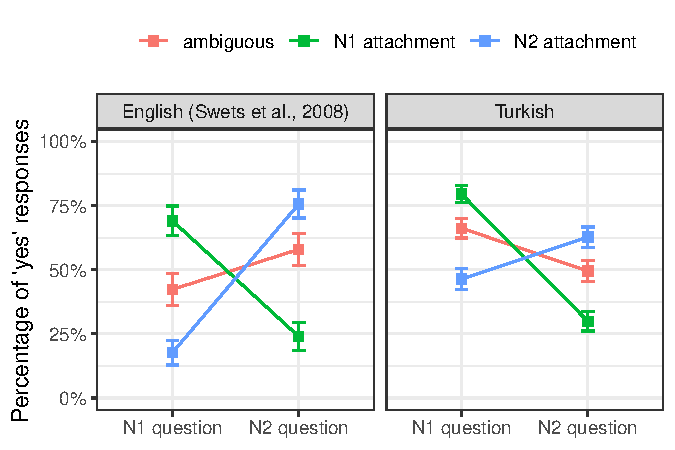
\includegraphics[width=7.5cm]{../figures/avg_perc.pdf}
\caption{Average percentates of \textit{'yes'} responses by attachment condition (color) and question type (x-axis). Error bars indicate 95\% within-subject CIs.}
\label{avg_perc}
\end{figure}


The average percentages of \textit{'yes'} responses in figure \ref{avg_perc} indicate a substantial number of errors in unambiguous experimental conditions, such as \textit{'no'}-responses to N1 questions and \textit{'yes'}-responses to N2 questions about N1 attachment sentences.

The average accuracy in answering questions about unambiguous sentences was $79\%$ $(SE=1.3)$
% N1: 72.6 (1.3); N2: 79.0 (1.2)
in Swets et al.'s English experiment, and $66.5\%$ $(SE=2.5)$
% N1: 74.8 (2.3); N2: 58.2 (2.6)
in the Turkish experiment. The difference is likely due to the fact that the former was conducted in a lab, while the latter was conducted online.

The question responses in ambiguous attachment conditions indicate an N2 attachment preference in the English as $58\%$ $(SE=2.1)$ of the response are compatible with N2 attachment (\textit{'yes'} responses to N2 questions and \textit{'no'} responses to N1 questions). Meanwhile, the Turkish data indicates an N1 preference as $58\%$ $(SE=1.9)$ of the question responses are compatible with an N1 interpretation of the sentence. In both cases, the preferred attachment option is \textit{local}, i.e., adjacent to the RC, which is consistent with prior research.

In spite of the fact that the estimates of the magnitude of the attachment preference are coincidentally equal, these numbers cannot be taken at face value because of the presence of a substantial number of erroneous responses in unambiguous conditions in both experiments. These responses suggest that not all N1- or N2-compatible responses indicate that the participant has successfully formed an N1- or N2 attachment interpretation of the sentence, as they may have been generated by the same extraneous cognitive process that generates erroneous responses in unambiguous attachment conditions. 
In the next section, we test two models of erroneous responses and then use them to quantify the actual strength of the attachment preference.

%... maybea:is att Both experiments are more likely to reflect on-line attachment preferences than pure offline studies, because participants read the sentence once, and didn't get the chance to re-read it unlike in typical offline experiments.


\section{MPT models of question-answering and attachment}

In accounting for the influence of extraneous cognitive processes, we considered two mechanisms that may generate erroneous question responses, and implemented both as multinomial processing tree (MPT) models \citep{BatchelderRiefer:1999} in order to the model with the better empirical fit to obtain less biased estimates of the attachment preferences in the ambiguous conditions, as indicated by question responses. 

MPT models offer a way to formalize hypotheses about how a mixture of several latent processes generates a categorical response 
\citep[cf.][ for an overview]{ErdfelderEtAl:2009}. Events involved in processing are represented as a probability tree, with hypothesized latent processes either occurring or not occurring at each junction, with each path corresponding to unique combinations of cognitive processes which give rise to a particular response, along with the probabilities of each path.
Importantly, this formalization provides a framework in which the probabilities of relevant latent processes can be estimated. We will use them to estimate the magnitude of the RC attachment preference in Turkish and English.

% Erdfelder et al., 2009 

% ... quite useful as measurement models, but not necessarily mechanistic models, 

%The simplest model we can use for that are called multinomial processing tree models and allow us to specify that each participant's responses are essentially a mixture of 'informed responses' and 'uninformed random button presses', and we can estimate the true preference by factoring out the bias introduced by random button presses.



\subsection{Model 1}


The first mechanism we considered as a potential explanation for erroneous responses is that people simply fail to attend to the stimulus or fail to perform the task of answering questions and simply press a random button. The logic of this account is illustrated in figure \ref{fig:mpt1}. The MPT schematic on top illustrates how events during processing of an N1 attachment sentence can unfold: On any given N1 attachment trial, a participant may be in an attentive state (probability: $a$), or in an inattentive state (probability $1-a$).

If the participant is in an attentive state throughout the trial (i.e., during reading and question answering), they will form a memory trace of the sentence they read, and later use it to correctly answer comprehension questions. This is illustrated in the top branch of the N1 attachment condition MPT schematic in figure \ref{fig:mpt1}, where \textit{'N1 response'} stands for \textit{'yes'} responses to N1 questions and \textit{'no'} responses to N2 questions.

If the participant is in an inattentive state at some point during the trial (i.e., during reading or question answering), they will either fail to form a memory trace of the sentence they read or will fail to use it to answer the comprehension question. On those occasions, they will respond \textit{'yes'} with probability $g$, and \textit{'no'} with probability $1-g$. This is illustrated in the bottom branch of the N1 attachment condition MPT schematic in figure \ref{fig:mpt1}.
 
As a result of these assumptions, the probability of a \textit{'yes'} response in the N1 attachment condition is as given in equation \ref{eq:m1pN1}, where $I_{N1}$ is an indicator variable which is $1$ for N1 comprehension questions and $0$ for N2 comprehension questions. 

The processing assumptions for the N2 attachment (middle, figure \ref{fig:mpt1}) condition and the ambiguous condition  (bottom, figure \ref{fig:mpt1}) follow a similar logic, with the probability of a \textit{'yes'} response given by equations \ref{eq:m1pN2} and \ref{eq:m1pAmb}. One important assumption about the hypothesized process for question-answering in ambiguous attachment conditions is that when readers are in an attentive state, they disambiguate ambiguous sentences either towards an N1 interpretation (with probability $h$) or an N2 interpretation (with probability $1-h$). We make no assumptions about whether that happens during reading or at the question answering stage.
% ... only yes responses as the only alternative

\begin{equation}
    p_{Y|N1} = a \cdot I_{N1} + (1-a) \cdot g
    \label{eq:m1pN1}
\end{equation}
\vspace{-0.5cm}
\begin{equation}
    p_{Y|N2} = a \cdot ( 1 - I_{N1} ) + (1-a) \cdot g
    \label{eq:m1pN2}
\end{equation}
\vspace{-0.8cm}
\begin{equation}
    p_{Y|A} = a \cdot   [ h  \cdot I_{N1} + (1 - h) \cdot (1-I_{N1}) ]  + (1-a) \cdot g 
    \label{eq:m1pAmb}
\end{equation}


Importantly, we make no claims as to what may bring on inattentiveness and when exactly it occurs (i.e., during reading or questions answering). We do speculate, however, that it may be brought on by distractions in the environment, mind-wandering (\cite[e.g.,][]{Smallwood:2011}), or (temporary) fatigue. However, an important prediction of this account is that this process should affect the different attachment conditions to the same degree, as its rate shouldn't depend on the attachment condition. 


\begin{center}
\begin{figure}
% <!-- \resizebox{7cm}{!}{ -->
% <!-- \begin{minipage}[t][5cm][b]{0,5\textwidth} -->
\begin{tiny}
\begin{forest}
for tree = {
% nodes
    draw, 
    align=center,
    minimum height=5ex,
    minimum width=3em,
    font=\linespread{0.84}\selectfont,
% tree
    grow'=0,
    parent anchor=east,
    child  anchor=west,
    s sep = 4mm,    
    l sep = 12mm, 
% edge
    edge = {semithick},
% level styles
if level = 0{}{rounded corners=2ex},
where n children=0{tier=level, sharp corners}{calign=edge midpoint},
% edge labels
EL/.style={edge label={node [pos=0.5, fill=white,
                             font=\scriptsize\sffamily,
                             inner sep=2pt] {$#1$}}
                    }
            }% end for tree
[,coordinate
  [N1\\ attachment\\ condition,no edge
        [attentive\\ state, EL=a
            ['N1\\ response']
        ]
        [inattentive\\ state, EL=1-a,
            ['yes'\\ response, EL=g ]
            ['no'\\ response, EL=1-g]
        ]
  ]
  [N2\\ attachment\\ condition,no edge
        [attentive\\ state, EL=a
            ['N2\\ response']
        ]
        [inattentive\\ state, EL=1-a,
            ['yes'\\ response, EL=g ]
            ['no'\\ response, EL=1-g]
        ]
  ]
  [ambiguous\\ attachment\\ condition,no edge
        [attentive\\ state, EL=a
            [N1\\ attachment, EL=h
                ['N1\\ response']
            ]
            [N2\\ attachment, EL=1-h
                ['N2\\ response']
            ]
        ]
        [inattentive\\ state, EL=1-a,
            ['yes'\\ response, EL=g ]
            ['no'\\ response, EL=1-g]
        ]
  ]
]
\end{forest}
\end{tiny}
% <!-- \end{minipage} -->
% <!-- } -->
\caption{An MPT model of question answering with equal error rates for (i) N1 attachment, (ii) N2 attachment, and (iii) ambiguous sentences. }
\label{fig:mpt1}
\end{figure}
\end{center}


\subsection{Model 2}

A second possible source of erroneous responses may be processes that do not affect all conditions equally across the board. For example, it could be that one of the two interpretations is more often successfully created during reading, or more often successfully recalled during question answering. Moreover, given that RC attachment is disambiguated via anaphor binding in both experiments, it is, in principle, possible that the preferred interpretation is usually attempted first, even in dispreferred attachment conditions, before that interpretation is rejected, and the correct dispreferred interpretation is constructed. As a result, the presence of a partial alternative structure could interfere with the retrieval of the correct structure during question answering \citep[e.g.,][]{Staub:2007}.


We formalized the assumption of different error rates associated with N1 and N2 attachment in the MPT model in figure \ref{fig:mpt2}. The hypothesized structure of unambiguous N1 and N2 attachment trials is similar to model 1 in figure \ref{fig:mpt1}. Each attachment process is associated with a probability of complete recollection certainty, $r_1$ and $r_2$, which reflect the probability that the correct sentence structure is (i) constructed during reading and (ii) later correctly recalled during the question-answering phase. If the correct sentence structure is constructed and later recalled with certainty, participants respond in accordance with the structure they constructed. Otherwise, they select a random response, i.e., \textit{'yes'} with a probability of $g$ and \textit{'no'} with a probability of $1-g$.
The probability of a \textit{'yes'} response for all attachment conditions is given in equations \ref{eq:m2pN1}, \ref{eq:m2pN2}, \ref{eq:m2pAmb}.

Importantly, in the ambiguous condition (figure \ref{fig:mpt2}, bottom), the recollection certainty and recollection uncertainty nodes are nested under the RC attachment nodes because the probabilities of the recollection certainty and uncertainty states depend on which RC attachment was chosen.
One way to interpret this model structure is that while there are (i) causes of recollection uncertainty which apply to all conditions equally and which affect processing across the board with probability $a \leq min(r_1, r_2)$, as well as (ii) additional attachment condition-specific causes of recollection uncertainty which affect processing with probability $r_1-a$ in when an N1 attachment is adopted, and with probability $r_2-a$ when N2 attachment adopted. However, all these sources of recollection uncertainty are assumed to lead to the same guessing behavior. Thus, the model in \ref{fig:mpt2} subsumes the model in \ref{fig:mpt1}. 

\begin{equation}
p_{Y|N1} = r_1 \cdot I_{ N1 } + (1-r_1) \cdot g
\label{eq:m2pN1}
\end{equation}
\vspace{-0.5cm}
\begin{equation}
p_{Y|N2} = r_2 \cdot (1 - I_{N1}) +  (1-r_2) \cdot g
\label{eq:m2pN2}
\end{equation}
\vspace{-0.5cm}
\begin{equation}
p_{Y|A} =  h  \cdot p_{Y|N1} + (1-h) \cdot p_{Y|N2}
%\begin{aligned}
% \\
%             &  
%\end{aligned}
\label{eq:m2pAmb}
\end{equation}


\section{Method}

We implemented both MPT models in \textit{brms} and \textit{rstan} \citep{R-brms, rstan} in R \citep{R-base} according to equations \ref{eq:m1pN1}-\ref{eq:m2pAmb}. We fitted the models to each experiment separately, using $4$ MCMC chains with $1,000$ warm-up and $3,000$ post-warm-up iterations.
For the sake of computational convenience, we estimated all model parameters on the logit scale, and in the following, we will use $\theta'$ to refer to the logit-transform of a parameter $\theta$.

We used mildly informative Gaussian priors for all logit-transformed parameters in both models: $h', g' \sim N(0,1)$, and $a, r_1, r_2 \sim N(0,1)$.

\begin{center}
\begin{figure}[h!]
% <!-- \resizebox{7cm}{!}{ -->
% <!-- \begin{minipage}[t][5cm][b]{0,5\textwidth} -->
%\hspace{-3cm}
\begin{tiny}
\begin{forest}
for tree = {
% nodes
    draw, 
    align=center,
    minimum height=5ex,
    minimum width=3em,
    font=\linespread{0.84}\selectfont,
% tree
    grow'=0,
    parent anchor=east,
    child  anchor=west,
    s sep = 4mm,    
    l sep = 12mm, 
% edge
    edge = {semithick},
% level styles
if level = 0{}{rounded corners=2ex},
where n children=0{tier=level, sharp corners}{calign=edge midpoint},
% edge labels
EL/.style={edge label={node [pos=0.5, fill=white,
                             font=\scriptsize\sffamily,
                             inner sep=2pt] {$#1$}}
                    }
            }% end for tree
[,coordinate
  [N1\\ attachment\\ condition,no edge
        [recollection\\ certainty, EL=r_{1}
            ['N1\\ response']
        ]
        [recollection\\ uncertainity, EL=1-r_{1},
            ['yes'\\ response, EL=g ]
            ['no'\\ response, EL=1-g]
        ]
  ]
  [N2\\ attachment\\ condition,no edge
        [recollection\\ certainty, EL=r_{2}
            [N2\\ response]
        ]
        [recollection\\ uncertainity, EL=1-r_{2},
            ['yes'\\ response, EL=g ]
            ['no'\\ response, EL=1-g]
        ]
  ]
  [ambiguous\\ attachment\\ condition,no edge
      [N1\\ attachment,EL=h
            [recollection\\ certainty, EL=r_{1}
                [N1\\ response]
            ]
            [recollection\\ uncertainity, EL=1-r_{1},
                ['yes'\\ response, EL=g ]
                ['no'\\ response, EL=1-g]
            ]
      ]
      [N2\\ attachment,EL=1-h
            [recollection\\ certainty, EL=r_{2}
                [N2\\ response]
            ]
            [recollection\\ uncertainity, EL=1-r_{2},
                ['yes'\\ response, EL=g ]
                ['no'\\ response, EL=1-g]
            ]
      ]
  ]
]
\end{forest}

\end{tiny}
% <!-- \end{minipage} -->
% <!-- } -->
\caption{An MPT model of question answering with different error rates for N1 attachment and N2 attachment processes.
}
\label{fig:mpt2}
\end{figure}
\end{center}

To account for individual differences in all parameters, we used hierarchical models with by-subject intercepts for all parameters, where each participant $k$'s responses were modeled as a function of population-level parameters $\theta$ with subject subject-level adjustments $\delta_{\theta,k}$, with $\theta_k' = \theta' + \delta_{{\theta'},k}$, where the by-subject adjustments are  distributed as $\delta_{{\theta'},k} \sim N(0, \sigma_{\theta'})$.

% ($a_k, h_k, g_k, r_1_k, r_2_k$), where $k$  
% to-do: link to the anonymized github repo
% The code and data can be found in the git repo here:

\section{Model Comparison}

Figures \ref{post_pred_ahg} and \ref{post_pred_r1r2hg} show the average percentages of \textit{'yes'} responses by experiment alongside 95\% posterior predictive intervals generated by, models 1 and 2, respectively.

\begin{figure}
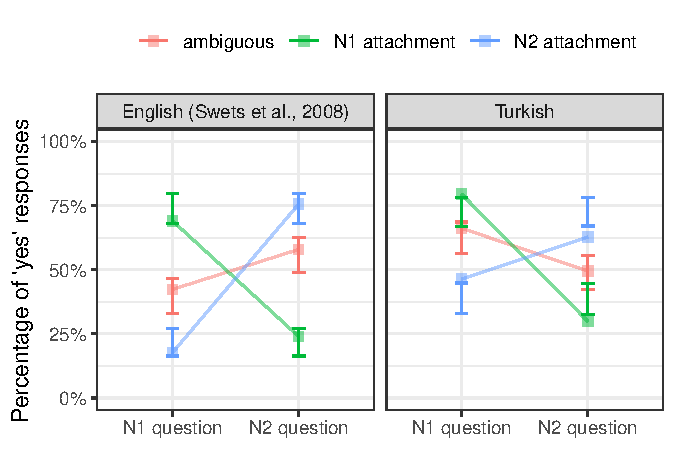
\includegraphics[width=7cm]{../figures/post_pred_ahg.pdf}
\caption{Average percentages of \textit{'yes'} responses and $95\%$ posterior prediction intervals based on model 1 by attachment condition and question type.}
\label{post_pred_ahg}
\end{figure}


Figure \ref{post_pred_ahg} shows that although model 1 could approximate the experimental findings to a degree, it systematically overestimated the proportion of responses compatible with the preferred RC attachment (N2 in English, N1 in Turkish) in both unambiguous conditions: For example, in the N1 attachment condition in English, the number of \textit{'yes'} responses to N1 questions and \textit{'no'} responses to N2 questions were slightly overestimated. Similarly, in the N2 attachment condition in Turkish, the model underestimated the percentage of \textit{'yes'} responses to N1 questions and \textit{'no'} responses to N2 questions.  Figure \ref{post_pred_r1r2hg} shows that model 2 appears to have fewer systematic deviations, and appears to fit the data quite well.

In order to compare the candidate models more formally, we computed each model's expected log pointwise predictive density ($\widehat{elpd}$) using PSIS-LOO-CV \citep{loo} as an estimate of the model's out-of-sample performance. Table \ref{tab:model_comp} shows the $\widehat{elpd}$ estimates, the differences between models in $\widehat{elpd}$ as well as their respective standard errors. Given that both $\Delta\widehat{elpd}$ estimates are relatively large relative to their standard errors, they both point towards model 2 as having better out-of-sample performance.
This finding suggests that the two attachment processes are affected by the error-generating process to different degrees.



\begin{figure}
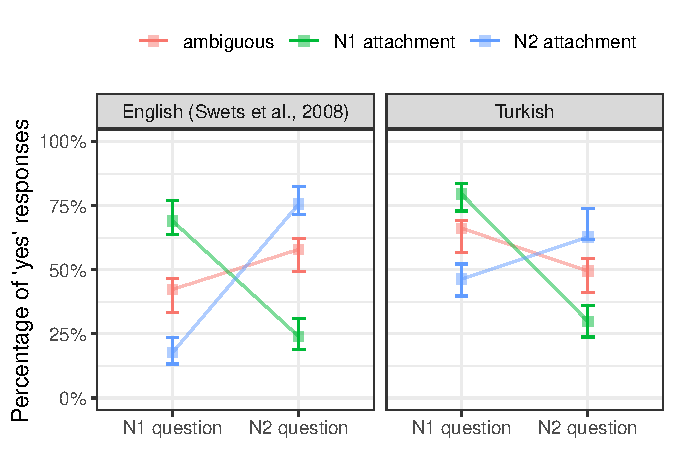
\includegraphics[width=7cm]{../figures/post_pred_r1r2hg.pdf}
\caption{Average percentages of \textit{'yes'} responses and $95\%$ posterior prediction intervals based on model 2 by attachment condition and question type.}
\label{post_pred_r1r2hg}
\end{figure}

\begin{table}
\centering
\begin{tabular}{lcc}
\hline
        & English & Turkish \\
\hline
        & $\widehat{elpd}$ & $\widehat{elpd}$ \\
\hline
model 1 & $-511.3$ $(18.1)$ & $-796.4$ $(15.0)$ \\
model 2 & $-469.4$ $(14.8)$ & $-750.5$ $(13.5)$ \\
\hline
 &  &  \\
 & $\Delta\widehat{elpd}$ & $\Delta\widehat{elpd}$ \\
\hline
model 2-1 & $41.9$ $(11.6)$ & $45.9$ $(9.3)$
\end{tabular}
\caption{Estimates of expected log pointwise predictive density ($\widehat{elpd}$) by model for each experiment and differences between model $\widehat{elpd}$s. Standard errors in brackets. }
\label{tab:model_comp}
\end{table}


\begin{figure}
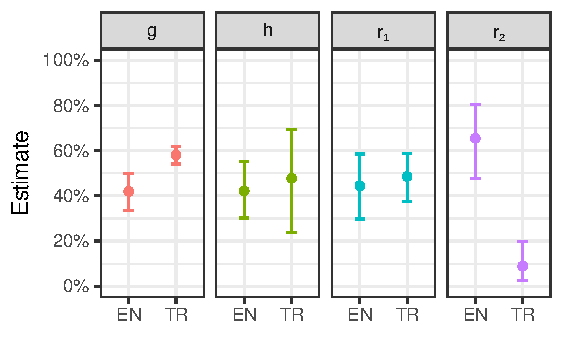
\includegraphics[width=7cm]{../figures/estimates_r1r2hg.pdf}
\caption{Population parameter estimates and 95\% credible intervals for all four parameters of model 2 ($g, h, r_1, r_2$) for both experiments, English (EN) and Turkish (TR). }
\label{estimates_r1r2hg}
\end{figure}


\section{Discussion}

Having established model 2 as an adequate model of RC attachment in the context of question-answering, we used its parameter estimates to understand the pattern of responses than accuracy rates: Figure \ref{estimates_r1r2hg} shows the population parameter estimates and 95\% credible intervals for all four parameters of model 2. In addition to difference in the guessing bias $g$ between experiments, it also shows a rather small difference between experiments in the estimates of attachment preference parameter $h$, which represents the probability with which the parser adopts an N1 attachment interpretation over an N2 attachment structure in ambiguous attachment conditions. The estimates of the N1 attachment probability were $42\%$ $(CrI=[30; 55])$ for the English experiment and $48\%$ $(CrI=[24; 70])$ for the Turkish experiment. While the estimate for English is consistent with an N2 attachment preference, the estimate for Turkish indicates no clear preference.

\textit{But why does the estimate of the attachment preference parameter $h$ for Turkish lead to different conclusions than the percentage of N1 responses in the ambiguous condition?} 
Generally speaking, the discrepancy is due to the fact that the percentage of N1 response conflates several parameters. 
In this particular instance, the explanation seems to lie in the very low estimate of the parameter $r_2$ ($9\%$, $CrI=[3; 20]$), which indicates that N2 attachment structures were unlikely to be successfully constructed or recalled. A possible reason for this is that even on trials resulting in an N2 interpretation, the parser always attempts to construct an N1 attachment structure first because, in Turkish, unlike in English, potential attachment sites are processed sequentially. As a result, a remnant of the N1 attachment interpretation may interfere with the retrieval of the memory trace of the N2 attachment interpretation. 
It appears likely, that as a result of retrieval failure, participants would resort to guessing, which in turn should lead to a substantial number of erroneous responses following N2 attachment sentences or ambiguous sentences which were disambiguated towards N2 attachment.
% NOTE: I feel like these above-mentioned errors should be predominantly 'yes' responses. This can probably be tested by yet another model?

Whatever really the true source of higher error rates in the N2 attachment conditions in the Turkish experiment, our MPT analysis suggests that what appears as a weak N1 attachment preference in our Turkish experiment is actually a consequence of a large number of \trials{guessing trials} associated with N2 attachment. It appears that when an N1 attachment structure is adopted in ambiguous sentences, participants often give an N1 response on approximately $50\%$ of the trials and guess on the remaining trials. In contrast, when an N2 attachment structure is adopted, participants tend to correctly give an N2 response on only approximately $10\%$ of the trials and guess on the remainder. Assuming that N1 structures are adopted approximately $50\%$ percent of the time, the expected proportion of N1 responses in the ambiguous condition is $60\%$, which is close to the $58\%$ we obtained.

In sum, our analysis shows that (i) the N2 attachment preference in the English experiment appears to hold up even when guessing trials are taken into account, and (ii) that what appears to be an N1 attachment preference is readily explained by processing difficulty associated with processing and recalling N2 attachment structures in Turkish.





%\begin{figure}
%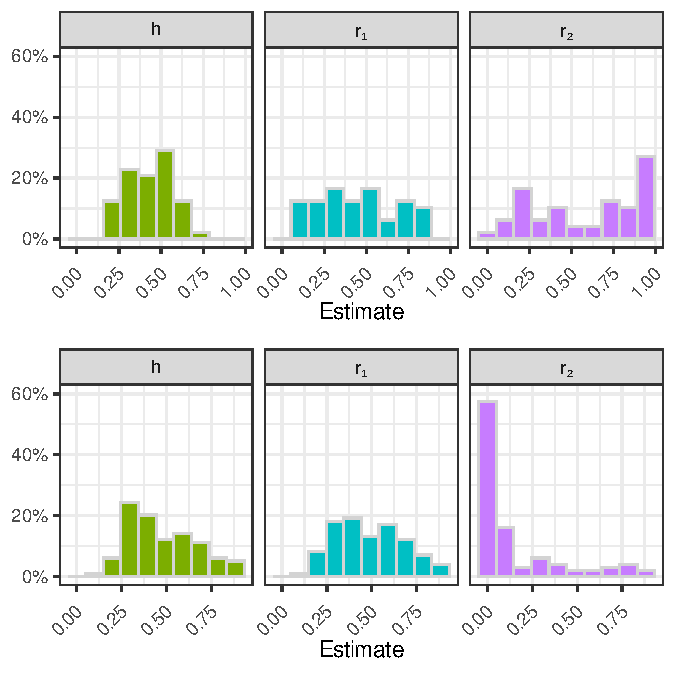
\includegraphics[width=7cm]{../figures/estimates_r1r2hg_bysubj.pdf}
%\caption{Histogram of by-participant MAP parameter estimates ($\theta + \delta_{\theta,k}$) for the parameters $h$, $r_1$, $r_2$ for the English (top) and Turkish (bottom).}
%\label{estimates_r1r2hg_bysubj}
%\end{figure}


\section{Summary}

In this paper, we have discussed a previously neglected source of bias and variability that may affect studies of attachment preferences and interpretation preferences more generally. We proposed an MPT-based analysis method which allows to de-confound parameters of theoretical importance from nuisance parameters such as the guessing rate. We tested two variants of the MPT-based model, and demonstrated that this method can provide further insight into the processes underlying participants' answering behavior as well as their attachment preferences. 



%Well, it's because they several sources of variation which the MPT can help us separate. Importantly, using averages to estimate attachment preferences amounts to just using model 1 with a=1, which is clearly an inadequate model, given that model 1 with a free $a$ parameter is already quite bad, and given that the estimates of $r_1$ and $r_2$ are quite far away from 1.

%- Talk about how this method might be assumption-ladden, but so is the method of using averages - and those are definitely wrong.



%\section*{Acknowledgements}
%We would like to thank Müge Tuncer for her help with the design of the Turkish experiment, as well as for writing most of the experimental stimuli, as well as Kadernur Akpınar for her assistance with the comprehension questions for the Turkish experiment.
%We would also like to thank Benjamin Swets for kindly sharing the \citet{SwetsEtAl:2008} experimental data.

\bibliography{custom} % anthology,
\bibliographystyle{acl_natbib}

%\appendix
%\section{Example Appendix}
%\label{sec:appendix}
%This is an appendix.

\end{document}
